\clearpage
% \setcounter{page}{1}
\maketitlesupplementary



% \input{tables/DL3DV_details}
\section{FLOPs for View Synthesis Transformers}
\label{supp:flop-calcs}

In this section, we explain how we calculated FLOP consumption for all models. Additionally, we show that in our regime, the MLP cost is most significant. In a vision transformer, there are three contributions to the FLOPs:
\begin{itemize}
    \item Initial patchifying + tokenization layers (negligible)
    \item Transformer blocks: attention.
    \item Transformer blocks: MLP and projections.
\end{itemize}
The first is negligible as it is a single linear layer at the start. Letting $n$ be the number of tokens and $d$ the transformer dimension, for each self-attention transformer block, the following are the FLOPs consumed by the attention, projection, and MLP layers:
\begin{align}
    \computeMLP, \computeProj &\propto n d^2 \\
    \computeAttn &\propto n^2 d
\end{align}
Thus, the total FLOPs consumed for a transformer block are of the form
\begin{equation}
    \compute{} = A n^2 d + B nd^2,
\end{equation}
where $A$ is $4$ while $B$ is $16$ in the self-attention case, so even at the smallest model size list (\suppref{supp:size-list}), $\frac{Bnd^2}{An^2d} \approx 4 \cdot \frac{384}{512} \approx 3$, meaning in most cases our MLP / linear projection FLOPs take up a large majority. For SVSM's cross-attention decoder, the formula becomes a little more complicated as there are separate $n_{\text{ctxt}}$ and $n_{\text{target}}$, but these remain on the same order of magnitude as $n$, so the same is true. 

For the decoder-only model, the number of tokens $n$ is given by
\begin{equation}
    n = (V_C + 1) \cdot \frac{H}{p} \cdot \frac{W}{p},
\end{equation}
where $p$ is the patch size and $H$ and $W$ are the width and height. For the SVSM encoder-decoder, the number of active tokens vary as 
\begin{equation}
    n_{\text{enc}} = V_C \cdot \frac{H}{p} \frac Wp, n_{\text{dec}} = V_T \cdot \frac Hp \cdot \frac Wp,
\end{equation}
So, for both models we can write down the MLP and attention complexities as:
\begin{align}
    \computeMLP^{(\text{LVSM})} &\propto V_T n \propto V_T (V_C + 1) \\
    \computeMLP^{(\text{SVSM})} &\propto n_{\text{enc}} + n_{\text{dec}} \propto V_C + V_T \\
    \computeAttn^{(\text{LVSM})} &\propto V_T n^2 \propto V_T (V_C + 1)^2 \\
    \computeAttn^{(\text{SVSM})} &\propto n_{\text{enc}}^2 + n_{\text{enc}}n_{\text{dec}} \propto V_C^2 + V_CV_T
\end{align}
For fixed $V_C$, we see that multiplying $V_T$ by an amount $k$ scales compute by exactly $k\times$ in LVSM, while it only scales compute by $\frac{kV_T + V_C}{V_T + V_C}$ in the SVSM case, which is where its advantage lies.

\begin{table}[t]
\centering
\begin{threeparttable}
% \vspace{-1\baselineskip}
\footnotesize            % <<— Increase font size here
\setlength{\tabcolsep}{4pt}  % <<— Reduce column padding to prevent wide table

% --- TABLE ---
\begin{tabular}{lcccccc}   % <<— Use tabular (not tabular*) to shrink width
\toprule

& \multicolumn{3}{c}{\textbf{Encoder}}
& \multicolumn{3}{c}{\textbf{Decoder}} \\
\cmidrule(lr){2-4} \cmidrule(lr){5-7}

\textbf{Params}
& \textbf{dim} & \textbf{dim\_head} & \textbf{n\_layers}
& \textbf{dim} & \textbf{dim\_head} & \textbf{n\_layers} \\
\midrule

% 15 & 384 & 64 & 3 & 384 & 64 & 3 \\
% 27 & 384 & 64 & 6 & 384 & 64 & 6 \\
% 35 & 384 & 64 & 8 & 384 & 64 & 8 \\
% 62 & 512 & 64 & 8 & 384 & 64 & 8 \\
% 79 & 512 & 64 & 8 & 512 & 64 & 12 \\
% 145 & 640 & 64 & 10 & 640 & 64 & 14 \\
% 226 & 768 & 64 & 10 & 768 & 64 & 16 \\
% 316 & 768 & 64 & 12 & 768 & 64 & 24 \\
% \hline
% \textbf{420} & 768 & 64 & 16 & 768 & 64 & 32 \\
% 740 & 1024 & 64 & 16 & 1024 & 64 & 32 \\

15M & 384 & 64 & 3 & 384 & 64 & 3 \\
27M & 384 & 64 & 6 & 384 & 64 & 6 \\
35M & 384 & 64 & 8 & 384 & 64 & 8 \\
62M & 512 & 64 & 8 & 384 & 64 & 8 \\
79M & 512 & 64 & 8 & 512 & 64 & 12 \\
145M & 640 & 64 & 10 & 640 & 64 & 14 \\
226M & 768 & 64 & 10 & 768 & 64 & 16 \\
316M & 768 & 64 & 12 & 768 & 64 & 24 \\
\hline
\textbf{420M} & 768 & 64 & 16 & 768 & 64 & 32 \\
740M & 1024 & 64 & 16 & 1024 & 64 & 32 \\


\bottomrule
\end{tabular}

\caption{\textbf{RealEstate10K $\boldsymbol{V_C}\mathbf{{=}2}$, SVSM Encoder-Decoder.} SVSM Encoder-Decoder model settings used to sweep scaling laws for the stereo ($V_C{=} 2$) novel view synthesis setting. \textbf{Bolded} is the row for the compute-matched, Pareto-optimal SVSM model compared against the 24-layer LVSM Decoder-only model.}
\label{tab:svsm-re10k-details}
\end{threeparttable}
\end{table}
\begin{table}[t]
\centering
\begin{threeparttable}

\footnotesize            % <<— Increase font size here
\setlength{\tabcolsep}{4pt}  % <<— Reduce column padding to prevent wide table

% --- TABLE ---
\begin{tabular}{lcccccc}   % <<— Use tabular (not tabular*) to shrink width
\toprule

& \multicolumn{3}{c}{\textbf{Encoder}}
& \multicolumn{3}{c}{\textbf{Decoder}} \\
\cmidrule(lr){2-4} \cmidrule(lr){5-7}

\textbf{Params}
& \textbf{dim} & \textbf{dim\_head} & \textbf{n\_layers}
& \textbf{dim} & \textbf{dim\_head} & \textbf{n\_layers} \\
\midrule

  8M & - & - & - & 384 & 64 & 3 \\
13M & - & - & - & 384 & 64 & 6 \\
22M & - & - & - & 512 & 64 & 6 \\
28M & - & - & - & 512 & 64 & 8 \\
53M & - & - & - & 640 & 64 & 10 \\
90M & - & - & - & 768 & 64 & 12 \\
118M & - & - & - & 768 & 64 & 16 \\
175M & - & - & - & 768 & 64 & 24 \\
275M & - & - & - & 896 & 64 & 28 \\

\bottomrule
\end{tabular}

\caption{\textbf{RealEstate10K $\boldsymbol{V_C}\mathbf{{=}2}$, LVSM Decoder-only.} LVSM Decoder-only model settings used to sweep scaling laws for the stereo ($V_C{=}2$) novel view synthesis setting.}
\label{tab:dec-only-re10k-details}
\vspace{-\baselineskip}
\end{threeparttable}
\end{table}





\section{Further Experimental Details}
\label{supp:exp-details}

\subsection{Training Details}

All models in this study are multi-view ViTs, following the design of LVSM~\citep{jin2024lvsm}. The main deviation is no layer index-dependent initialization. All layers are initialized with the same standard deviation. Instead, for stability, we apply a $1/\sqrt{L}$ multiplier on the residuals of all layers where $L$ is the depth of the transformer. Empirically, we find this to maintain stable training on the same learning rate across multiple transformer depths. 

All models are trained with the AdamW optimizer, with a peak learning rate of $4\text{e-}4$, $\beta_1 = 0.9$, $\beta_2 = 0.95$, and weight decay of $0.05$ on all parameters except LayerNorm weights, all following LVSM. We additionally warmup the learning rate for $3000$ steps in all models. 

All models are trained on $256\times 256$ resolution for both DL3DV and RealEstate10K. All models are trained with the same reconstruction metric used in~\citep{jin2024lvsm}. In particular, the loss is
\begin{equation}
    \mathcal L = \text{MSE}(I_T, \tilde I_T) + \lambda \cdot \text{Perceptual}(I_T,\tilde I_T),
\end{equation}
where we choose $\lambda = 0.5$ as our perceptual loss weight. 

We also have a few experiment specific details. For $V_C{=}2$, RealEstate10K, we sample our context and target views from a video index range from 25-192. For $V_C{>}2$, DL3DV, we sample our context and target views from a video index range of 16-24 as the baselines between consecutive frames in DL3DV are much wider. For effective batch tests under $V_C{=}4$ on DL3DV, we train each model for 100k iterations, while under $V_C{=}2$ on RealEstate10K, we train for less iterations (50k) to save compute resources. The trend is still clear even with the limited iterations. 

\begin{table}[t]
\centering
\begin{threeparttable}

\footnotesize            % <<— Increase font size here
\setlength{\tabcolsep}{4pt}  % <<— Reduce column padding to prevent wide table

% --- TABLE ---
\begin{tabular}{lcccccc}   % <<— Use tabular (not tabular*) to shrink width
\toprule

& \multicolumn{3}{c}{\textbf{Encoder}}
& \multicolumn{3}{c}{\textbf{Decoder}} \\
\cmidrule(lr){2-4} \cmidrule(lr){5-7}

\textbf{Params}
& \textbf{dim} & \textbf{dim\_head} & \textbf{n\_layers}
& \textbf{dim} & \textbf{dim\_head} & \textbf{n\_layers} \\
\midrule

15M & 384 & 64 & 3 & 384 & 64 & 3 \\
32M & 384 & 64 & 6 & 384 & 64 & 8 \\
85M & 512 & 64 & 10 & 512 & 64 & 12 \\
168M & 640 & 64 & 12 & 640 & 64 & 16 \\
280M & 768 & 64 & 12 & 768 & 64 & 20 \\
711M & 1024 & 64 & 24 & 1024 & 64 & 24 \\
\hline
\textbf{400M} & 768 & 64 & 24 & 768 & 64 & 24 \\

\bottomrule
\end{tabular}

\caption{\textbf{DL3DV $\boldsymbol{V_C}\mathbf{{=}4}$, SVSM Encoder-Decoder.} SVSM Encoder-Decoder model settings used to sweep scaling laws for the multi-view ($V_C > 2$) novel view synthesis setting. \textbf{Bolded} is the row for the compute-matched, Pareto-optimal SVSM model compared against the 24-layer LVSM Decoder-only model.}
\label{tab:svsm-dl3dv-details}
\end{threeparttable}
\end{table}

\begin{table}[t]
\centering
\begin{threeparttable}

\footnotesize            % <<— Increase font size here
\setlength{\tabcolsep}{4pt}  % <<— Reduce column padding to prevent wide table

% --- TABLE ---
\begin{tabular}{lcccccc}   % <<— Use tabular (not tabular*) to shrink width
\toprule

& \multicolumn{3}{c}{\textbf{Encoder}}
& \multicolumn{3}{c}{\textbf{Decoder}} \\
\cmidrule(lr){2-4} \cmidrule(lr){5-7}

\textbf{Params}
& \textbf{dim} & \textbf{dim\_head} & \textbf{n\_layers}
& \textbf{dim} & \textbf{dim\_head} & \textbf{n\_layers} \\
\midrule

8M & - & - & - & 384 & 64 & 3 \\
22M & - & - & - & 512 & 64 & 6 \\
43M & - & - & - & 640 & 64 & 10 \\
90M & - & - & - & 768 & 64 & 12 \\
175M & - & - & - & 768 & 64 & 24 \\
383M & - & - & - & 1024 & 64 & 30 \\

\bottomrule
\end{tabular}

\caption{\textbf{DL3DV $\boldsymbol{V_C}\mathbf{{=}4}$, LVSM Decoder-only.} LVSM Decoder-only model settings used to sweep scaling laws for the multi-view ($V_C > 2$) novel view synthesis setting.}
\vspace{-0.5cm}
\label{tab:dec-only-dl3dv-details}
\end{threeparttable}
\end{table}



\begin{figure}[!t]
    \centering
    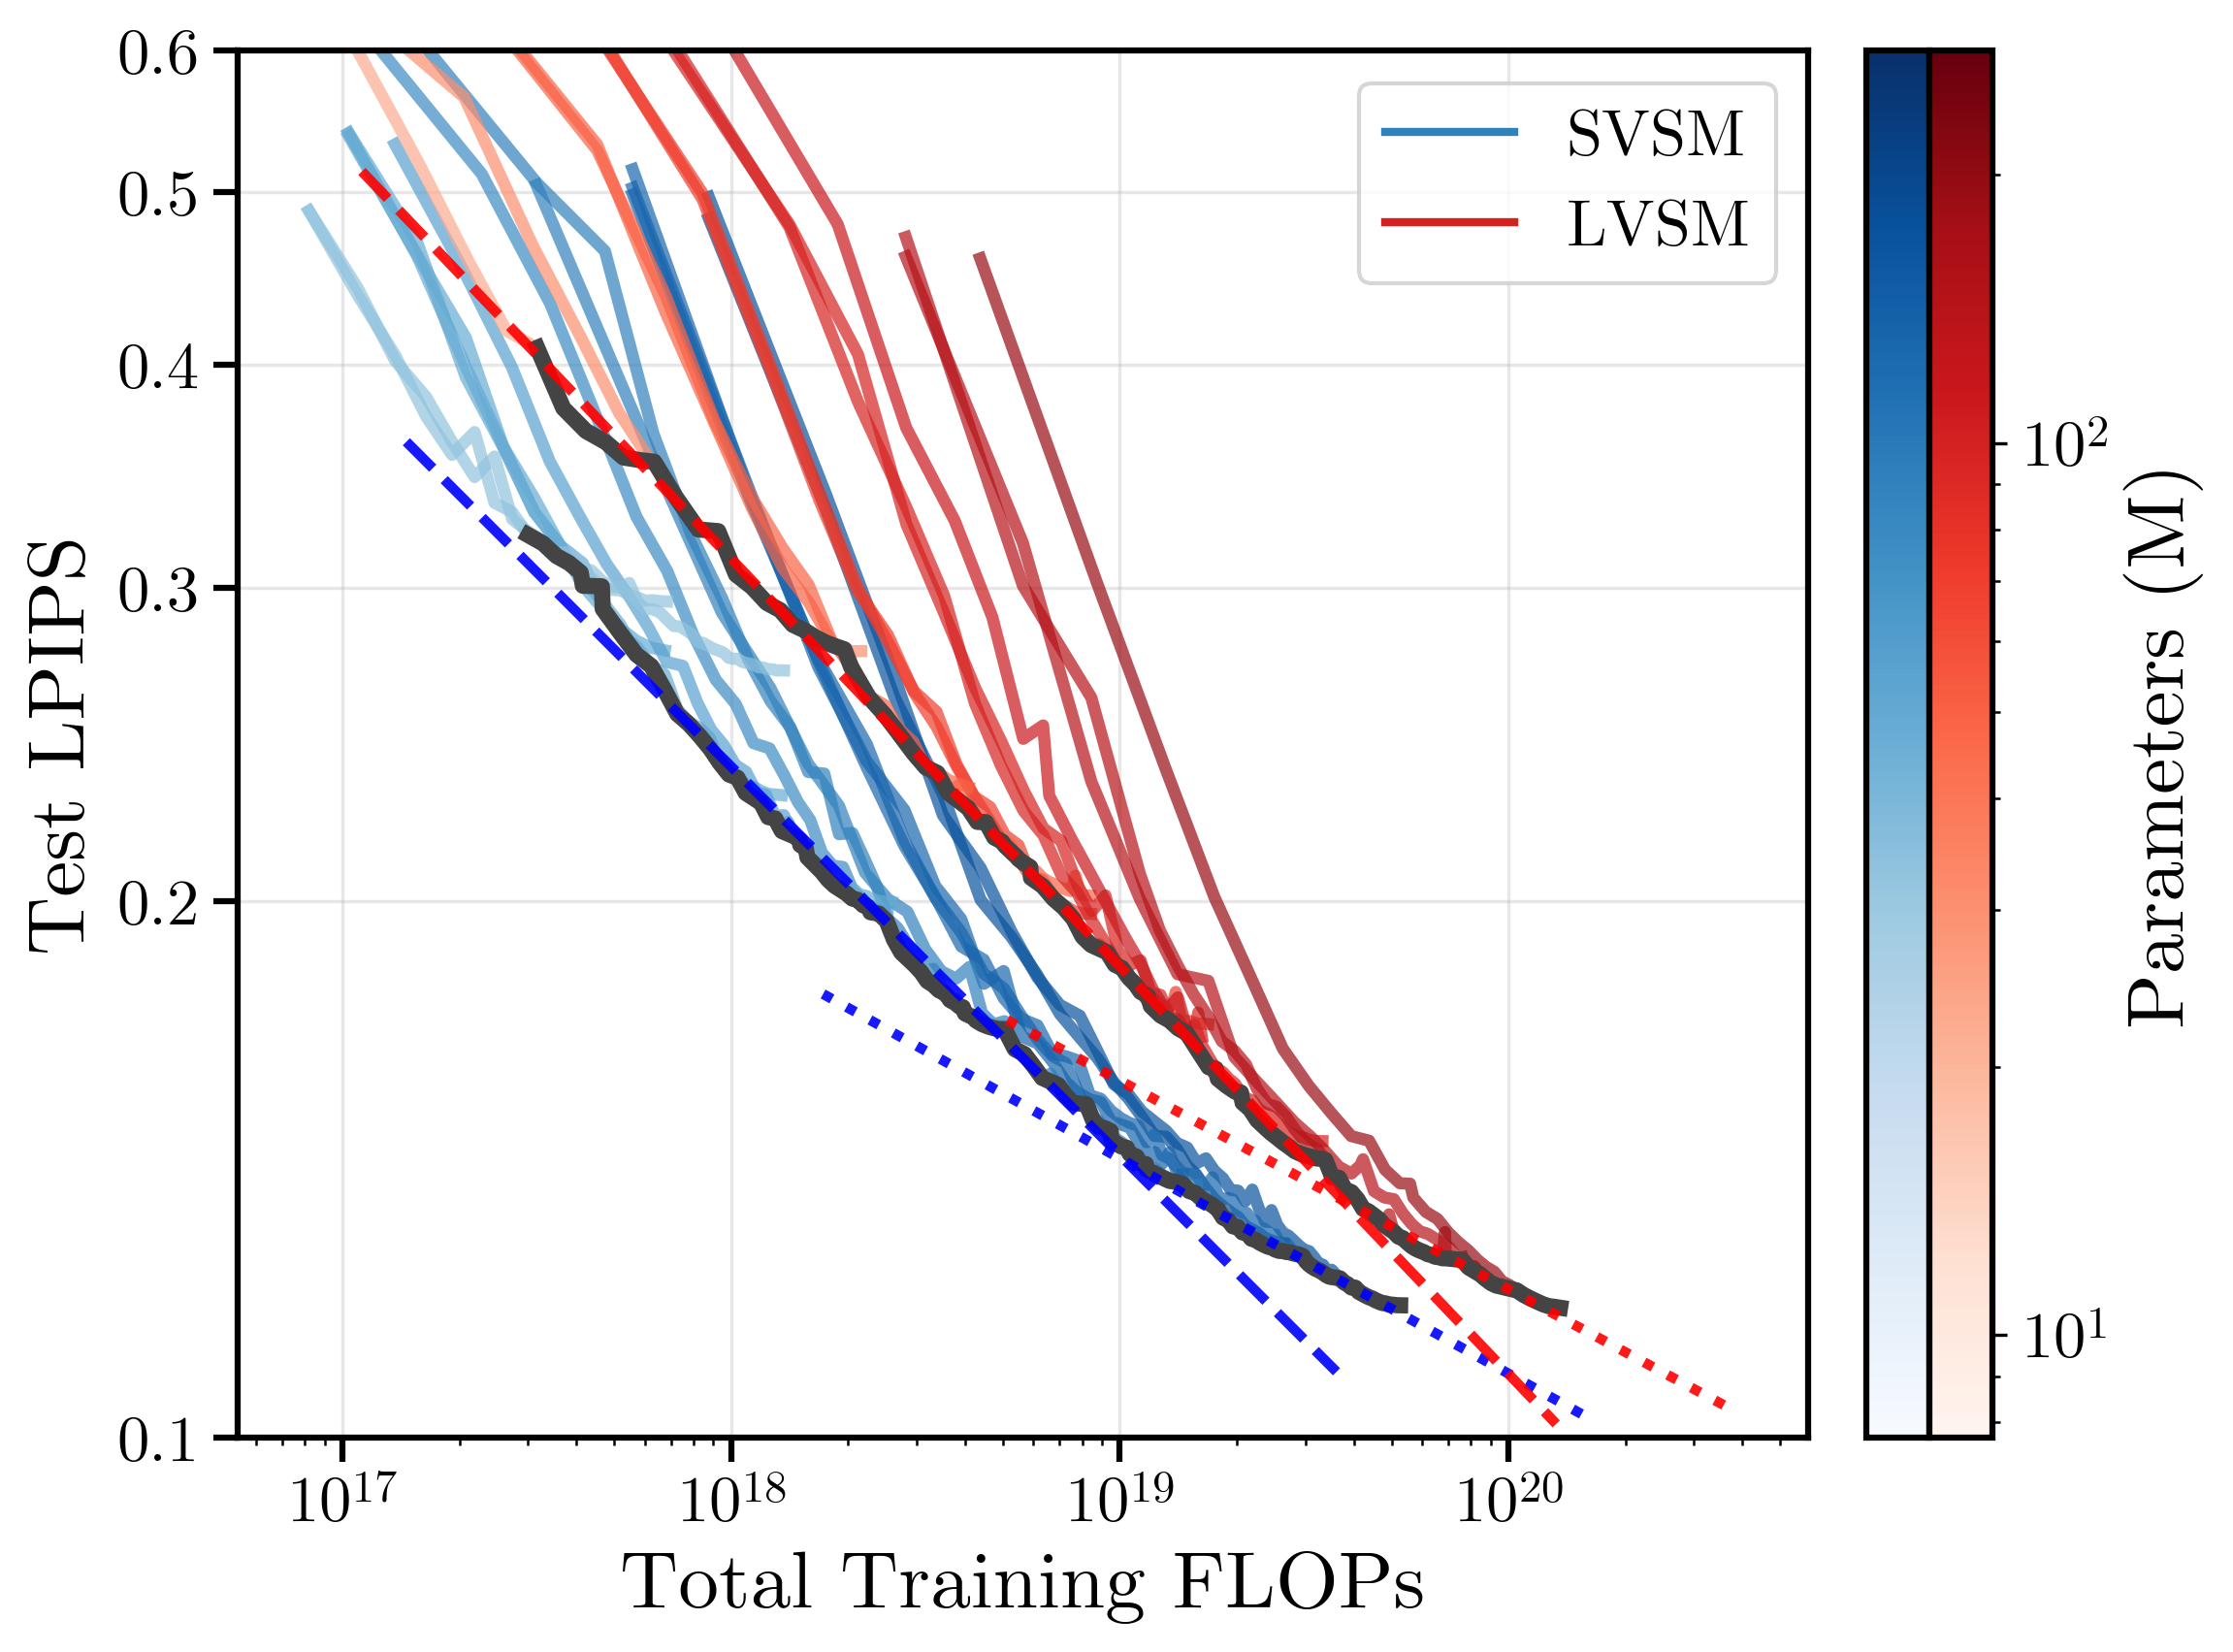
\includegraphics[width=\linewidth]{images/lpips_vs_flops_pareto_fits.png}
    \vspace{-0.5cm}
    \caption{\textbf{Linear Power Scaling Laws.} We fit scaling laws onto sections of the Pareto-frontiers of the model families. We see that both models have approximately the same slope in each of their corresponding sections, indicating equal scaling.}
    \vspace{-0.5cm}
    \label{fig:fits}
\end{figure}

\subsection{Rendering Speed Benchmarking}
\label{supp:rendering}

We benchmark all rendering on a single A6000 GPU. We found that due to some hardware configurations of our setup, when benchmarking with batch size $1$, all models would cap out at 30 fps, even when the width of each layer was increased or decreased, suggesting that there was some non-FLOP based bottleneck. To circumvent this, all models were tested with batch size $64$, which allowed the rendering FPS to properly reflect the forward pass FLOPs for each of the models. We still used $V_T = 1$ for all models, and report \begin{equation}
    \text{FPS} = \frac{B \cdot V_T}{t_{\text{iter}}} = \frac{B}{t_{\text{iter}}},
\end{equation}
where $t_{\text{iter}}$ is the iteration time for one batch. If higher $V_T$ was used (offline rendering), the rendering speed difference between our model and LVSM would be even larger.

\subsection{Model Size List for Scaling Sweeps}
\label{supp:size-list}

We trained a wide range of models across both families and both problem settings. Their sizes and hyperparameters are listed in tables \ref{tab:svsm-re10k-details}, \ref{tab:dec-only-re10k-details}, \ref{tab:svsm-dl3dv-details}, and \ref{tab:dec-only-dl3dv-details}. For the decoder-only model there is not much room for flexibility in terms of model hyperparameters -- we simply scale dimension up along with the layer count. For SVSM encoder-decoder we can flexibly allocate different amounts of compute to the encoder and the decoder. For low context view cases, we allocate more to the decoder as there are less complex relations amongst the context views and for higher context views we allocate similar amounts to the decoder as to the encoder. Empirically, we roughly found this to have better performance-per-compute, but we did not thoroughly study this split, so we leave this to future work. 

\section{Linear Fits on the Loss vs. Compute Frontiers}
\label{supp:fits}

Though the trend is not perfectly linear, we fit lines onto sections of  $P(\compute{}) \propto \compute{}^c$ in Fig.~\ref{fig:fits}, which show equal scaling between SVSM and LVSM. The actual coefficients are reported in \tabref{tab:lin-fits}, which have almost identical power law coefficients across the two model families.



\begin{table}[h]
\footnotesize
\centering
\begin{tabular}{lcc}
\toprule
\textbf{Model} & $c$ for $P > 0.14$ & $c$ for $P \le 0.14$ \\
\midrule
LVSM & -0.23 & -0.12 \\
SVSM & -0.22 & -0.12 \\
\bottomrule
\end{tabular}
\caption{\textbf{LPIPS vs. compute scaling coefficients.} As regressed from  \figref{fig:fits}, we find power law coefficients for LPIPS $P(\compute{}) \propto \compute{}^c$, and we report $c$ in this table for the first half, which is determined by test LPIPS loss greater than $0.14$ and the second half which is test LPIPS loss less than $0.14$.
\vspace{-1\baselineskip}
}
\label{tab:lin-fits}
\end{table}

\section{PRoPE Ablations}

We conduct a series of ablations on PRoPE~\cite{li2025cameras} in the multi-view setting in an attempt to elucidate the mechanism through which it enables scaling. One potential source of success is that the PRoPE SVSM design allows for the decoder to see the clean context poses, while vanilla SVSM does not. To test if this might be the cause for the success, we concatenated context plucker rays to the scene representation from the encoder. However, this has negligible impact (Tab.~\ref{tab:prope-abl-1}). Additionally, replacing PRoPE with GTA~\cite{miyato2023gta} showed negligible difference, indicating epipolar geometry is not crucial for viewcount scalability. Hence, we presume that the relative embeddings are the key, i.e., canonicalizing features to the target frame. Lastly, having PRoPE on just the decoder performs nearly as well as having PRoPE on both, indicating that the cross attention seems to benefit the most from the relative embedding inductive bias.

\begin{table}[h]
\footnotesize
\centering
\begin{tabular}{lccc}
\toprule
\textbf{Model} & \textbf{PSNR} (↑) & \textbf{SSIM} (↑) & \textbf{LPIPS} (↓)\\
\midrule
Vanilla SVSM & 23.50 & 0.727 & 0.254 \\
Vanilla w/ concat. pose & 23.47 & 0.726 & 0.254 \\
\midrule
PRoPE on Encoder & 23.61 & 0.733 & 0.249 \\
PRoPE on Decoder & 24.31 & 0.771 & 0.220\\
PRoPE on both & 24.62 & 0.782 & 0.210 \\
GTA on both & 24.63 & 0.782 & 0.207 \\
\bottomrule
\end{tabular}
\caption{\textbf{PRoPE ablations.} We vary where we apply PRoPE, try a different relative attention method (GTA), and also test pose information flow. GTA varies negligibly from PRoPE, indicating that epipolar geometry is not crucial, and the skip pose connection also has negligible impact, indicating that pose information flow is not responsible.}
\vspace{-1\baselineskip}
\label{tab:prope-abl-1}
\end{table}

% \begin{table}[h]
% \footnotesize
% \centering
% \begin{tabular}{lccc}
% \toprule
% \textbf{Model} & \textbf{PSNR} (↑) & \textbf{SSIM} (↑) & \textbf{LPIPS} (↓)\\
% \midrule
% PRoPE & 23.61 & 0.782 & 0.210 \\
% GTA & 24.63 & 0.782 & 0.207 \\
% \bottomrule
% \end{tabular}
% \caption{\textbf{Relative Attention is what matters.} asdf
% \vspace{-1\baselineskip}
% }
% \label{tab:prope-abl-2}
% \end{table}

\section{Compiled Scaling Results}

\begin{figure}[!t]
    \centering
    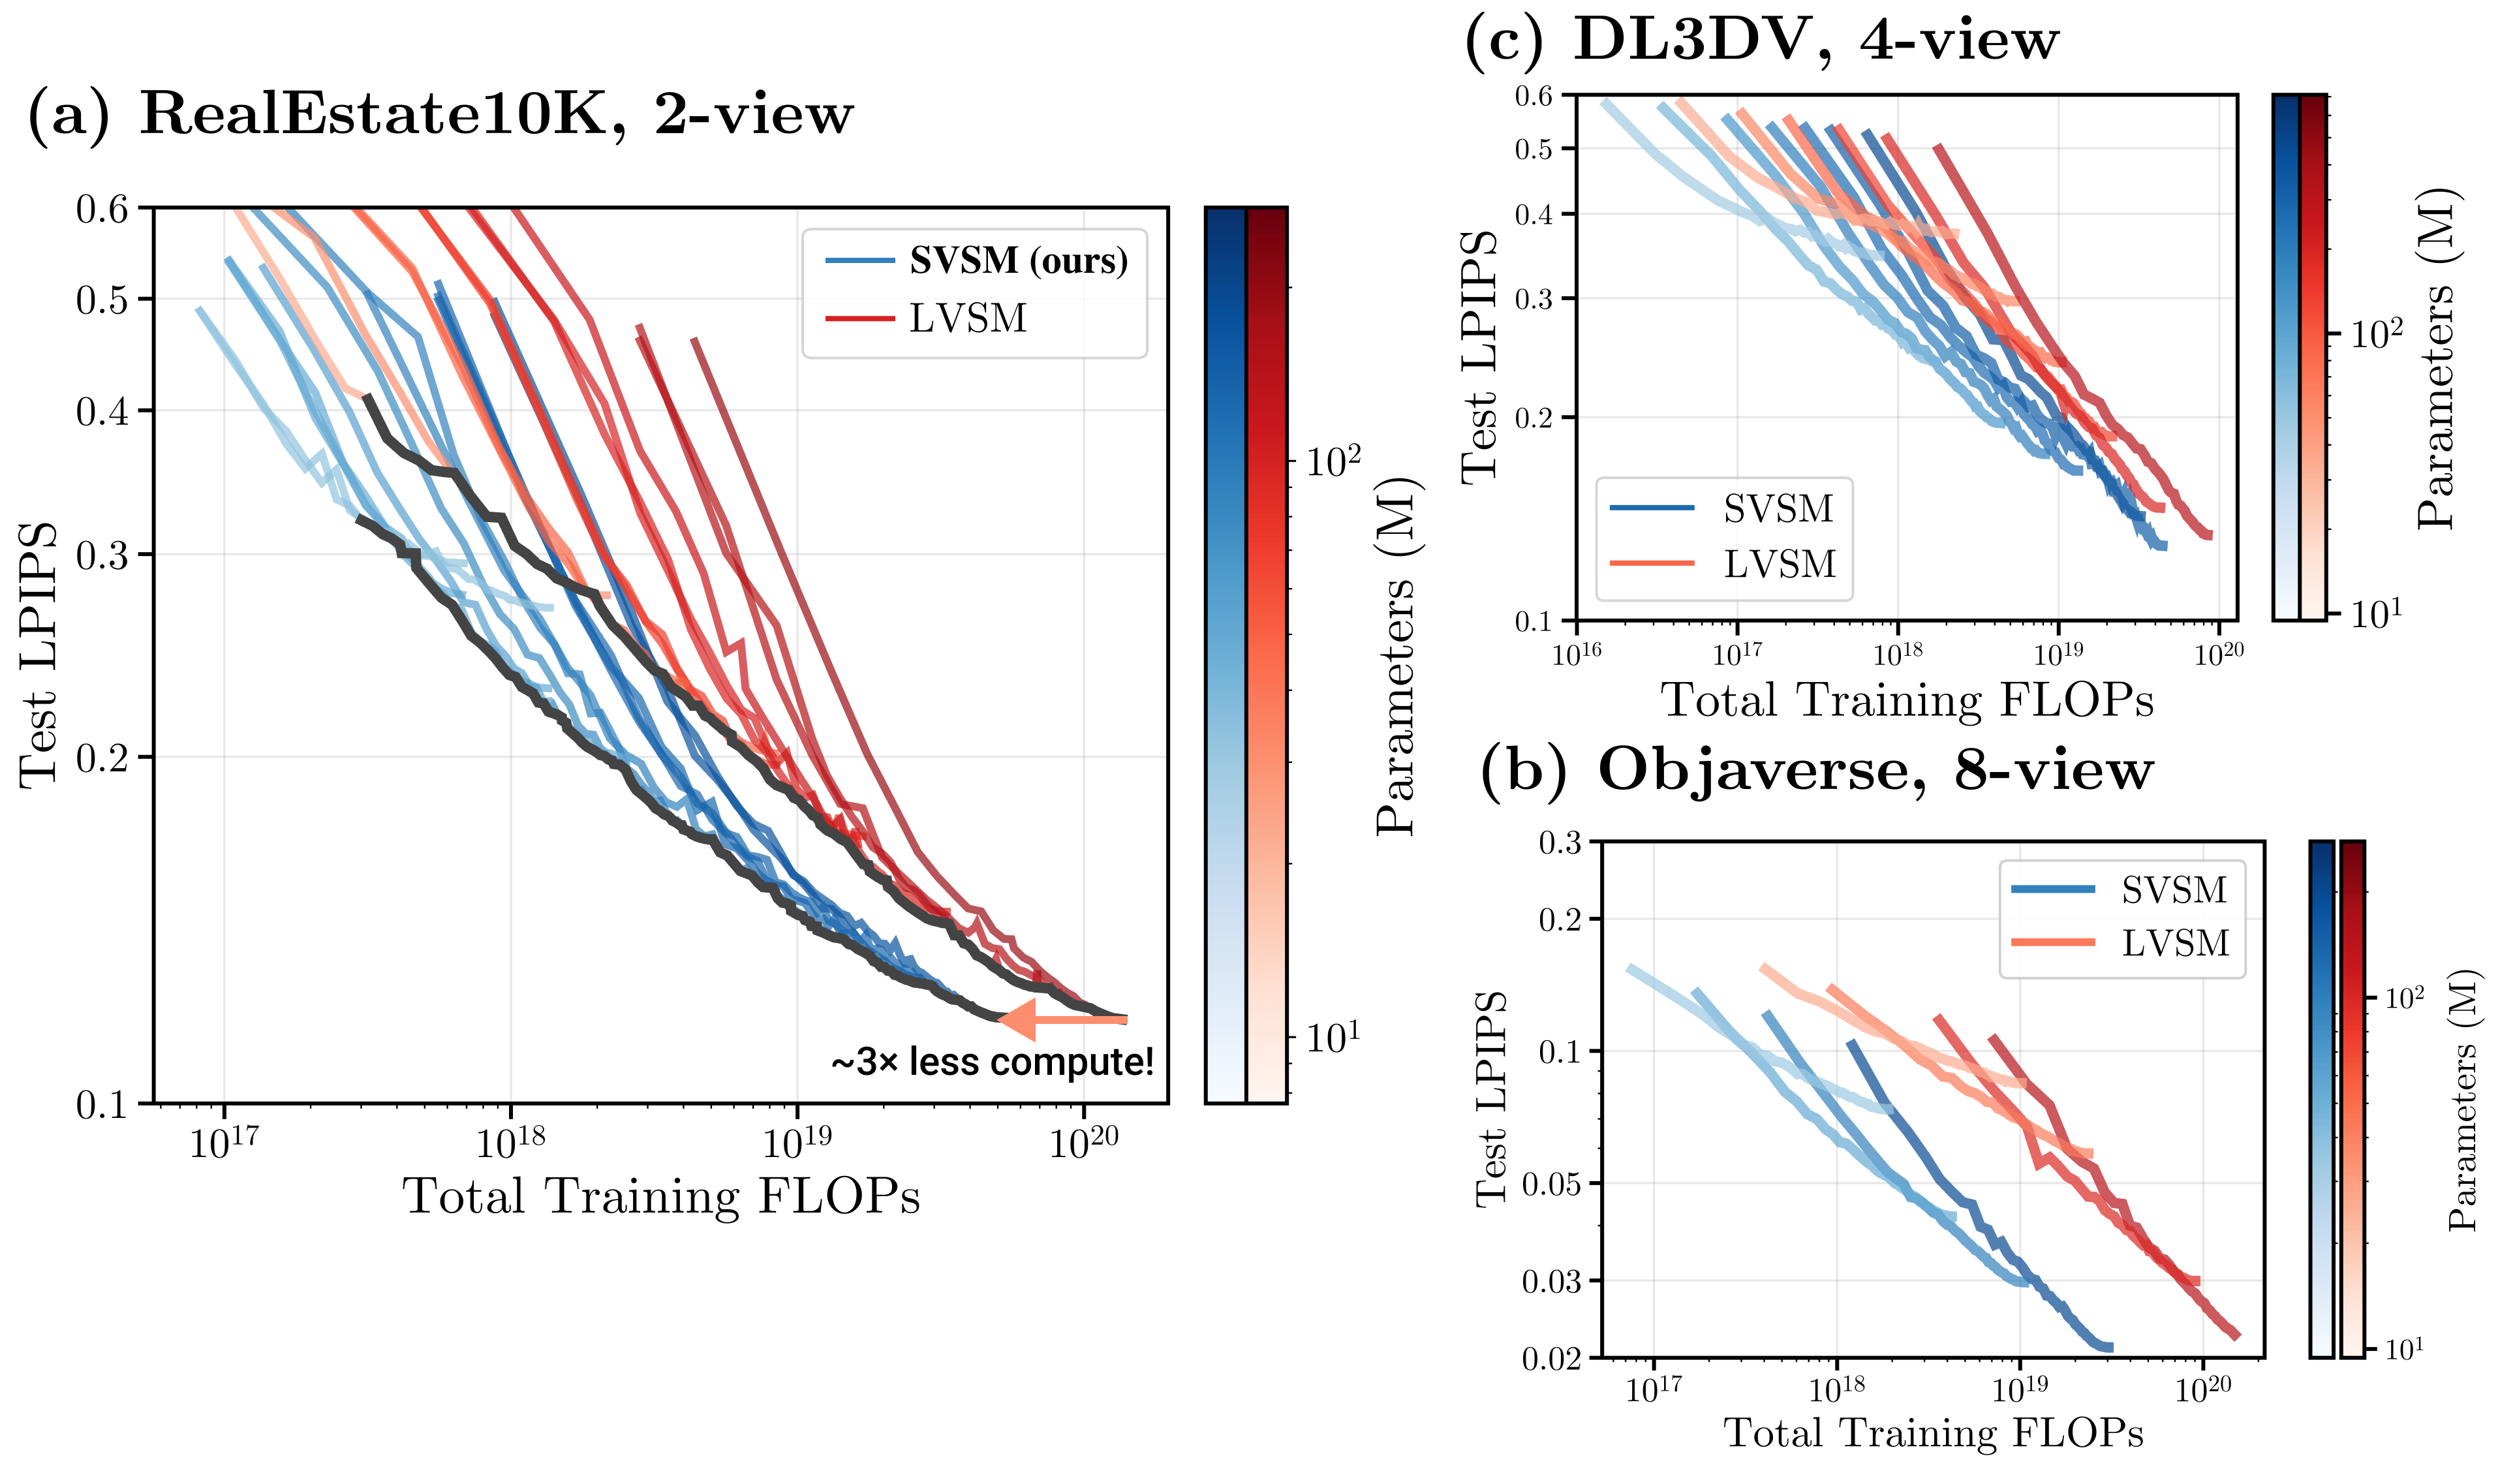
\includegraphics[width=\linewidth]{images/collected_scaling.png}
    \vspace{-0.5cm}
    \caption{\textbf{All Scaling Laws.} We collect scaling laws across the three datasets we tested on, and in all cases, SVSM is compute-optimal.}
    \vspace{-0.5cm}
    \label{fig:collected_scaling}
\end{figure}

We provide a collection of scaling results across RealEstate10K, DL3DV, and Objaverse across 2, 4, and 8 context views respectively in Fig.~\ref{fig:collected_scaling}. In all cases, SVSM (in blue) maintains a pareto advantage over LVSM decoder-only.

\section{Further Qualitative Results}
\label{supp:qual}

Lastly, we provide more qualitative results across various training compute budgets of 2 context view evaluations on RealEstate10K in Fig.~\ref{fig:supp-two-view-scale} and 4 context view evaluations on DL3DV in Fig.~\ref{fig:supp-four-view}. Multiview consistency of outputs is shown in Fig.~\ref{fig:qualitative-multiview-objaverse} on Objaverse.





% \section{Additional }

% \input{tables/3_grid}

\clearpage
\begin{figure*}[t]
    \centering
    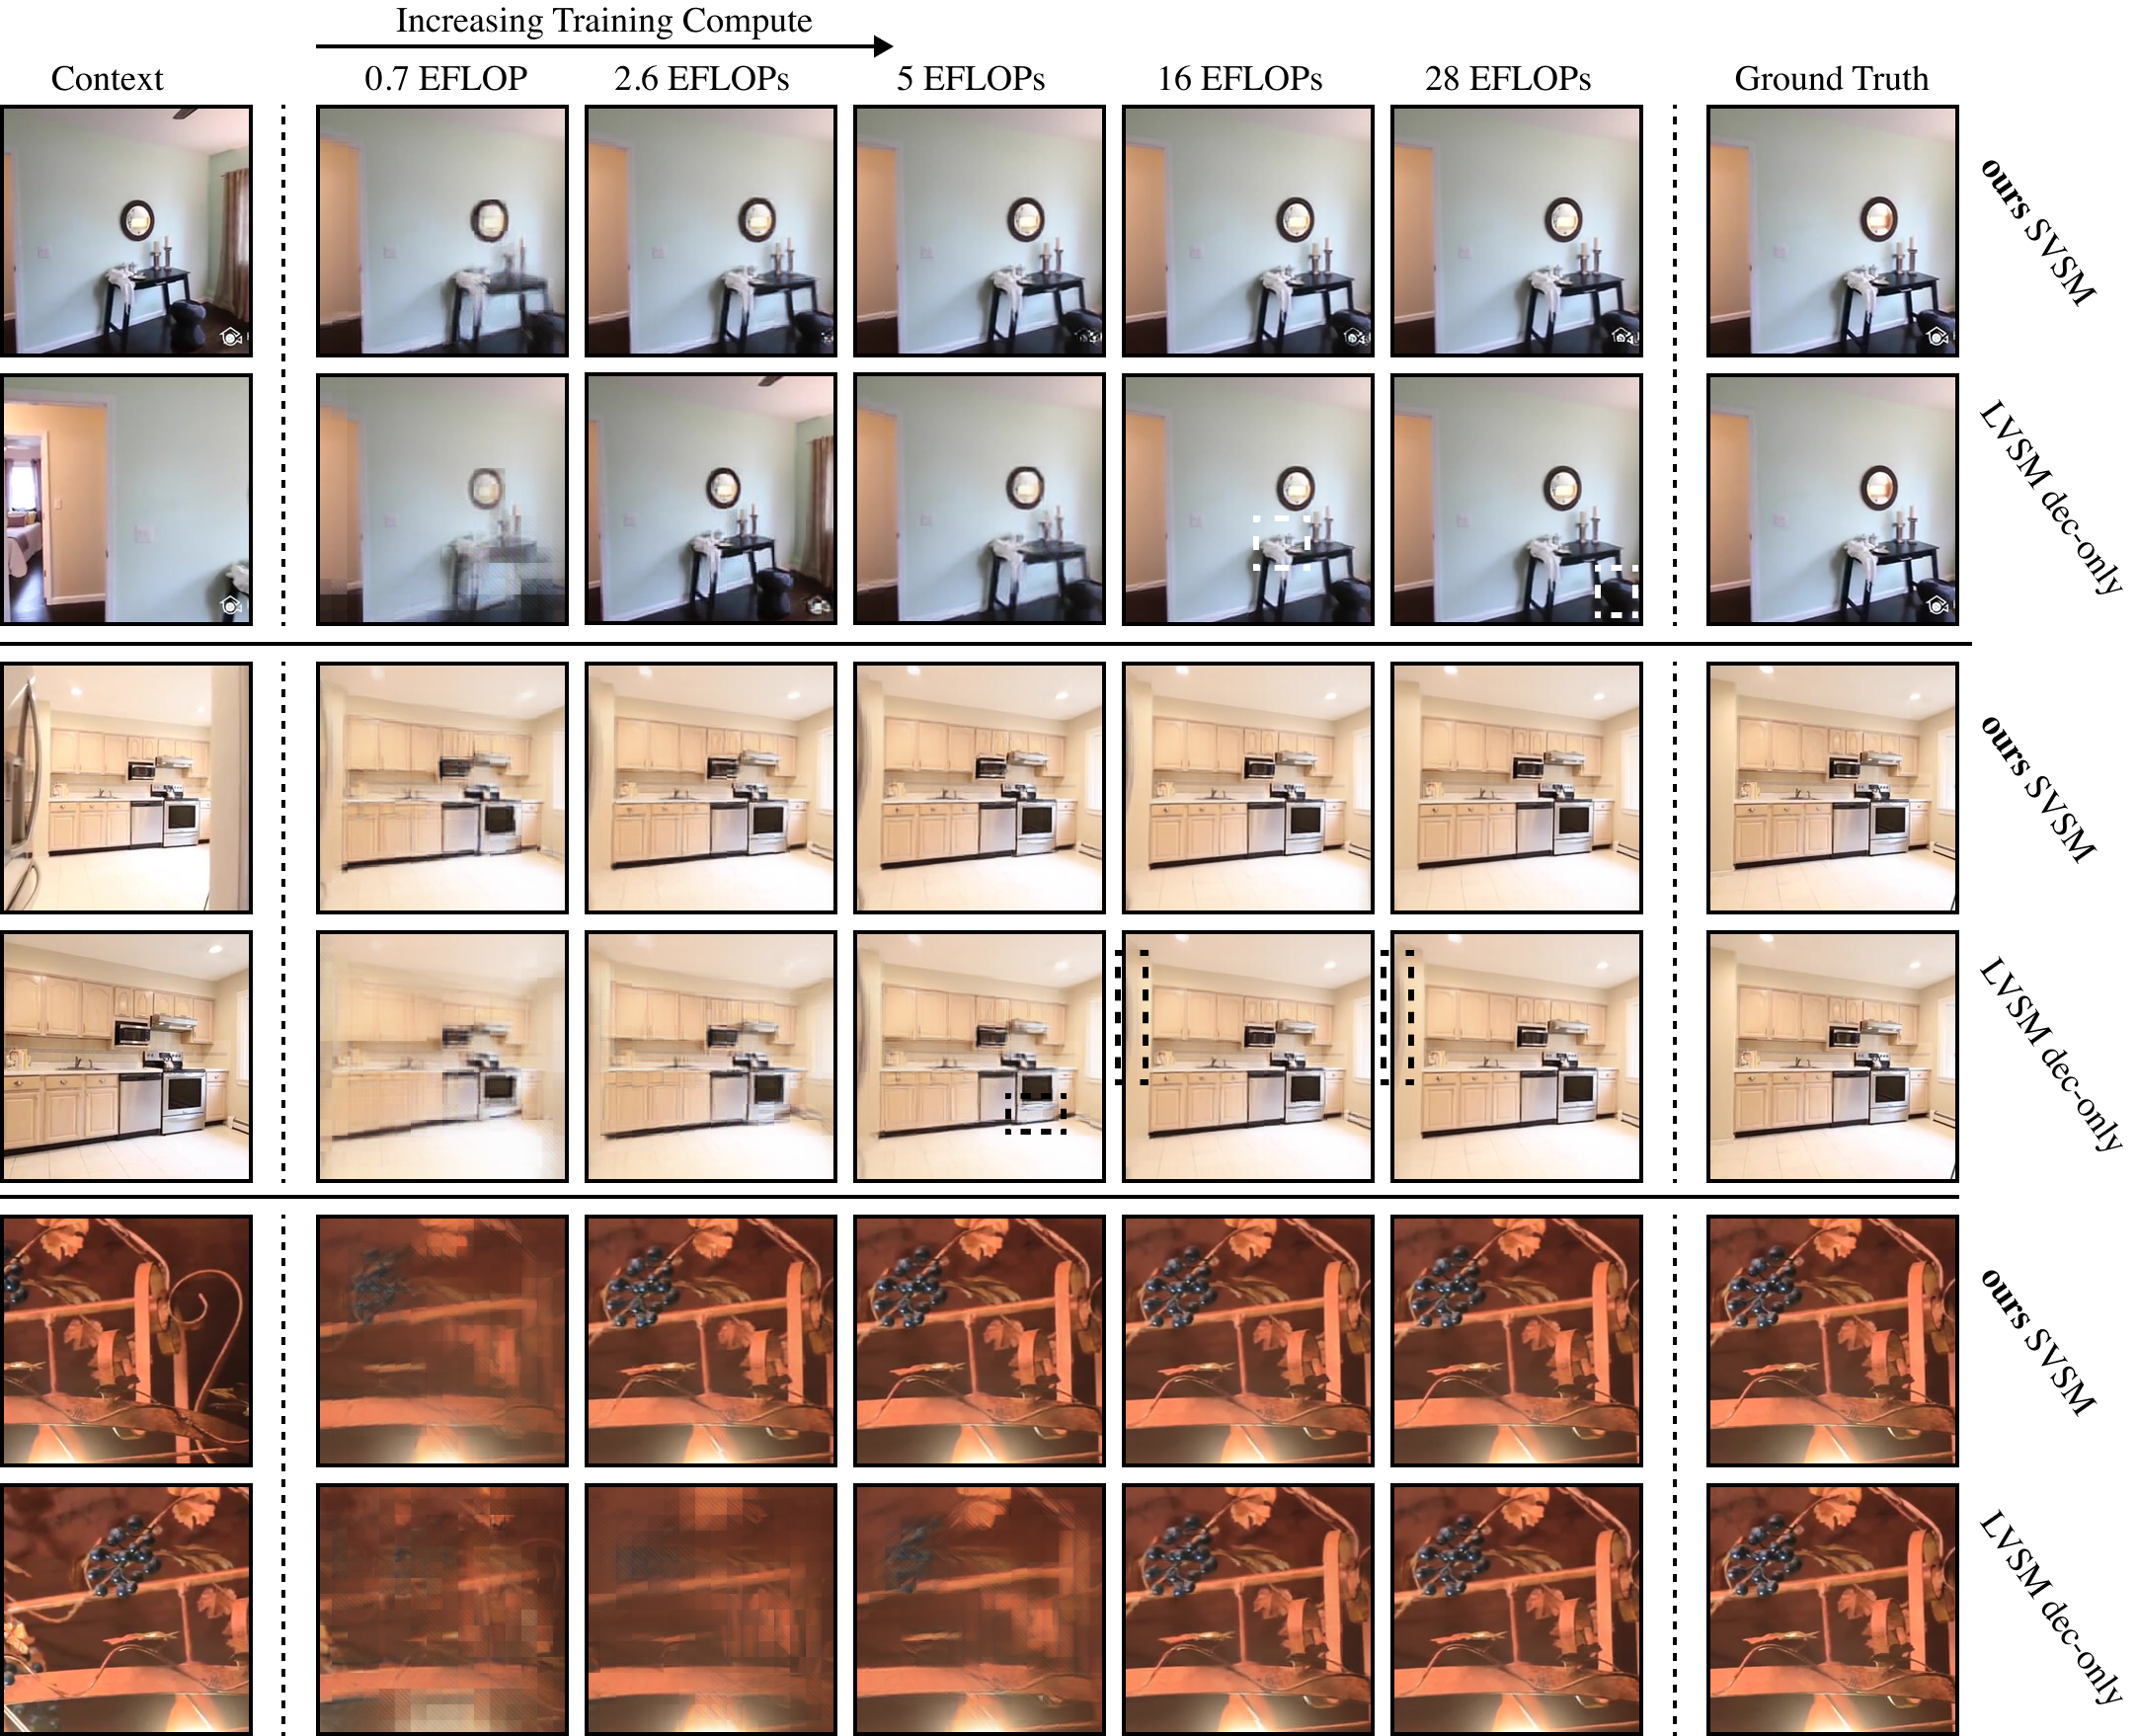
\includegraphics[width=\textwidth]{images/fixed_re10k_supp.png}
    \caption{Qualitative results on RE10K ($V_C{=}2$) across scale.}
    \label{fig:supp-two-view-scale}
\end{figure*}

% \input{figures/supp_two_view_final}




\begin{figure*}[t]
    \centering
    \includegraphics[width=\textwidth]{images/dl3dv_supp_fixed.png}
    \caption{Qualitative results on DL3DV ($V_C{=}4$) across scale.}
    \label{fig:supp-four-view}
\end{figure*}

\begin{figure*}[t]
    \centering
    \includegraphics[width=\textwidth]{images/objaverse_samples.png}
    \caption{
        Multiview consistency results on Objaverse ($V_C{=}8$).
    }
    \label{fig:qualitative-multiview-objaverse}
\end{figure*}








% \section{Rationale}
% \label{supp:rationale}
% % 
% Having the supplementary compiled together with the main paper means that:
% % 
% \begin{itemize}
% \item The supplementary can back-reference sections of the main paper, for example, we can refer to \cref{sec:intro};
% \item The main paper can forward reference sub-sections within the supplementary explicitly (e.g. referring to a particular experiment); 
% \item When submitted to arXiv, the supplementary will already included at the end of the paper.
% \end{itemize}
% % 
% To split the supplementary pages from the main paper, you can use \href{https://support.apple.com/en-ca/guide/preview/prvw11793/mac#:~:text=Delete%20a%20page%20from%20a,or%20choose%20Edit%20%3E%20Delete).}{Preview (on macOS)}, \href{https://www.adobe.com/acrobat/how-to/delete-pages-from-pdf.html#:~:text=Choose%20%E2%80%9CTools%E2%80%9D%20%3E%20%E2%80%9COrganize,or%20pages%20from%20the%20file.}{Adobe Acrobat} (on all OSs), as well as \href{https://superuser.com/questions/517986/is-it-possible-to-delete-some-pages-of-a-pdf-document}{command line tools}.